\documentclass{scrartcl}
\usepackage{amssymb}
\usepackage{amsmath}
\usepackage{tikz}
\usetikzlibrary{shapes.geometric}
\usetikzlibrary{positioning}	%for K5 of K5

\begin{document}

\hspace{1cm}
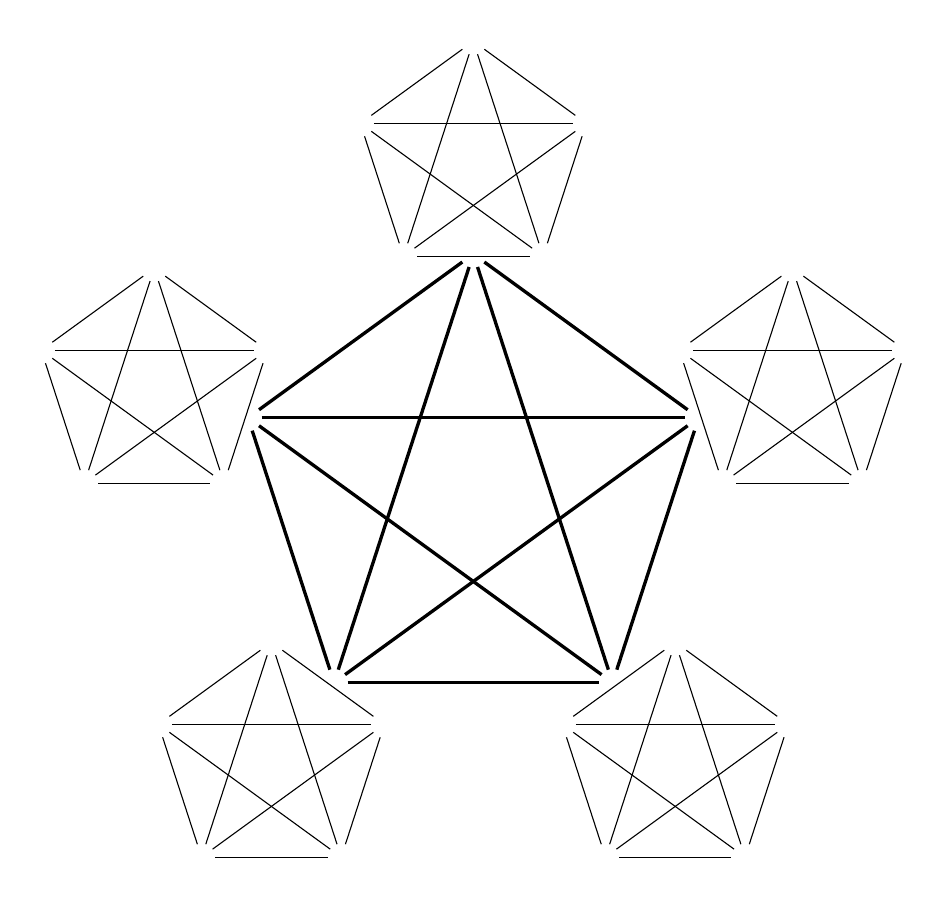
\begin{tikzpicture}[mystyle/.style={draw=white,shape=circle,fill=white}]
%meta-pentagon
\def\ngon{5}
\node[regular polygon,regular polygon sides=\ngon,minimum size=6cm] (p) {};
\foreach\x in {1,...,\ngon}{\node[mystyle] (p\x) at (p.corner \x){};}
\foreach\x in {1,...,\numexpr\ngon-1\relax}{
	\foreach\y in {\x,...,\ngon}{
		\draw[very thick] (p\x) -- (p\y);}}

%template for nodes
%\node at (p1) {{\large e}};
%\node at (p5) {{\large o}};
%\node at (p4) {{\large d}};		
%\node at (p3) {{\large r}};
%\node at (p2) {\hspace{-0.1cm}{\large m}};

%top vertex (p1)
\def\ngon{5}
\node[regular polygon,regular polygon sides=\ngon,minimum size=3cm,above = -0.2cm of p1] (t) {};
\foreach\x in {1,...,\ngon}{\node[mystyle] (t\x) at (t.corner \x){};}
\foreach\x in {1,...,\numexpr\ngon-1\relax}{
	\foreach\y in {\x,...,\ngon}{
		\draw (t\x) -- (t\y);}}

%top-right (p5)
\def\ngon{5}
\node[regular polygon,regular polygon sides=\ngon,minimum size=3cm,above right=-0.7cm and 0.1cm of p5] (TR) {};
\foreach\x in {1,...,\ngon}{\node[mystyle] (TR\x) at (TR.corner \x){};}
\foreach\x in {1,...,\numexpr\ngon-1\relax}{
	\foreach\y in {\x,...,\ngon}{
		\draw (TR\x) -- (TR\y);}}

%top-left (p2)
\def\ngon{5}
\node[regular polygon,regular polygon sides=\ngon,minimum size=3cm,above left=-0.7cm and 0.1cm of p2] (TL) {};
\foreach\x in {1,...,\ngon}{\node[mystyle] (TL\x) at (TL.corner \x){};}
\foreach\x in {1,...,\numexpr\ngon-1\relax}{
	\foreach\y in {\x,...,\ngon}{
		\draw (TL\x) -- (TL\y);}}

%bottom-right (p4)
\def\ngon{5}
\node[regular polygon,regular polygon sides=\ngon,minimum size=3cm,below right=0cm and -0.2cm of p4] (BR) {};
\foreach\x in {1,...,\ngon}{\node[mystyle] (BR\x) at (BR.corner \x){};}
\foreach\x in {1,...,\numexpr\ngon-1\relax}{
	\foreach\y in {\x,...,\ngon}{
		\draw (BR\x) -- (BR\y);}}

%bottom-left (p2)
\def\ngon{5}
\node[regular polygon,regular polygon sides=\ngon,minimum size=3cm,below left=0cm and -0.2cm of p3] (BL) {};
\foreach\x in {1,...,\ngon}{\node[mystyle] (BL\x) at (BL.corner \x){};}
\foreach\x in {1,...,\numexpr\ngon-1\relax}{
	\foreach\y in {\x,...,\ngon}{
		\draw (BL\x) -- (BL\y);}}
\end{tikzpicture}


\vspace{2cm}


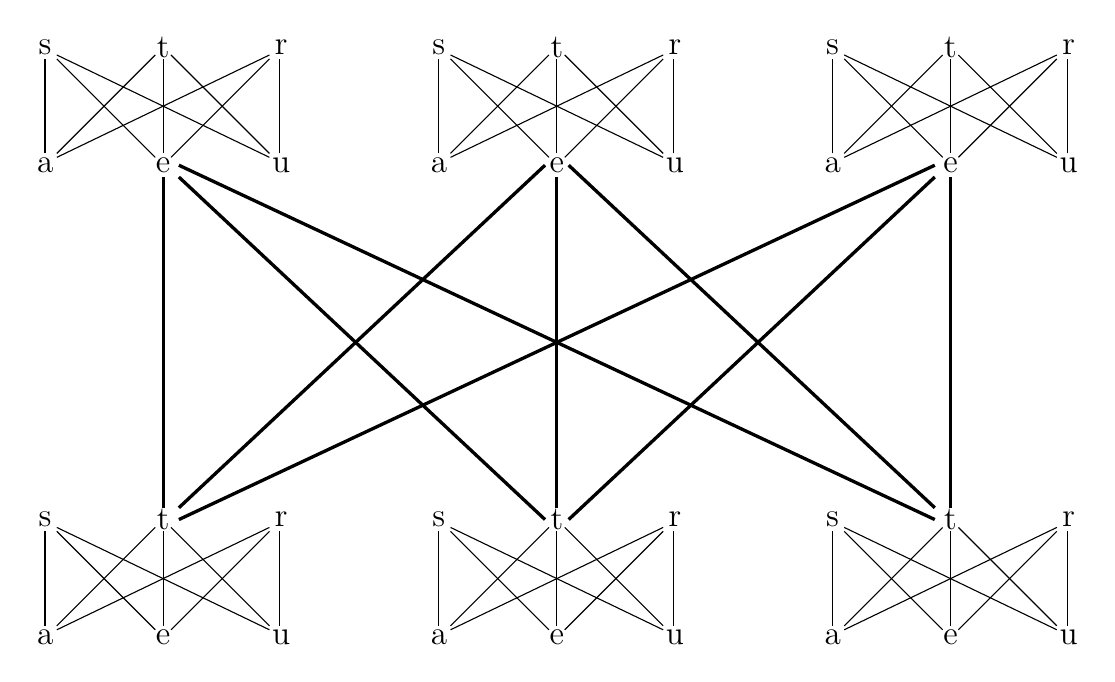
\begin{tikzpicture}		%meta-K3,3
%top-left - letters
\node at (-1.5,1.5) {{\large s}};
\node at (0,1.5) 	{{\large t}};
\node at (1.5,1.5) 	{{\large r}};
\node at (-1.5,0) 	{{\large a}};
\node at (0,0) 		{{\large e}};
\node at (1.5,0) 	{{\large u}};
%top-left - lines
\draw (-1.5,0.15)--(-1.5,1.35);	%a--s
\draw (0,0.15)--(0,1.35);		%e--t
\draw (1.48,0.15)--(1.48,1.35);	%u--r
%
\draw (-0.1,0.1)--(-1.35,1.35);	%e--s
\draw (0.1,0.1)--(1.35,1.35);	%e--r
%
\draw (-0.1,1.4)--(-1.35,0.15);	%t--a
\draw (0.1,1.4)--(1.35,0.15);	%t--u
%
\draw (-1.35,0.1)--(1.35,1.4);	%a--r
\draw (1.35,0.1)--(-1.35,1.4);	%u--s

%top-mid - letters
\node at (3.5,1.5) {{\large s}};
\node at (5,1.5) 	{{\large t}};
\node at (6.5,1.5) 	{{\large r}};
\node at (3.5,0) 	{{\large a}};
\node at (5,0) 		{{\large e}};
\node at (6.5,0) 	{{\large u}};
%top-mid - lines
\draw (3.5,0.15)--(3.5,1.35);	%a--s
\draw (5,0.15)--(5,1.35);		%e--t
\draw (6.48,0.15)--(6.48,1.35);	%u--r
%
\draw (4.9,0.1)--(3.65,1.35);	%e--s
\draw (5.1,0.1)--(6.35,1.35);	%e--r
%
\draw (4.9,1.4)--(3.65,0.15);	%t--a
\draw (5.1,1.4)--(6.35,0.15);	%t--u
%
\draw (3.65,0.1)--(6.35,1.4);	%a--r
\draw (6.35,0.1)--(3.65,1.4);	%u--s

%top-right - letters
\node at (8.5,1.5)  {{\large s}};
\node at (10,1.5) 	{{\large t}};
\node at (11.5,1.5) {{\large r}};
\node at (8.5,0) 	{{\large a}};
\node at (10,0) 	{{\large e}};
\node at (11.5,0) 	{{\large u}};
%top-right - lines
\draw (8.5,0.15)--(8.5,1.35);	%a--s
\draw (10,0.15)--(10,1.35);		%e--t
\draw (11.48,0.15)--(11.48,1.35);	%u--r
%
\draw (9.9,0.1)--(8.65,1.35);	%e--s
\draw (10.1,0.1)--(11.35,1.35);	%e--r
%
\draw (9.9,1.4)--(8.65,0.15);	%t--a
\draw (10.1,1.4)--(11.35,0.15);	%t--u
%
\draw (8.65,0.1)--(11.35,1.4);	%a--r
\draw (11.35,0.1)--(8.65,1.4);	%u--s

%bottom-left - letters
\node at (-1.5,-4.5) {{\large s}};
\node at (0,-4.5) 	 {{\large t}};
\node at (1.5,-4.5)  {{\large r}};
\node at (-1.5,-6) 	 {{\large a}};
\node at (0,-6) 	 {{\large e}};
\node at (1.5,-6) 	 {{\large u}};
%bottom-left - lines
\draw (-1.5,-5.85)--(-1.5,-4.65);	%a--s
\draw (0,-5.85)--(0,-4.65);			%e--t
\draw (1.48,-5.85)--(1.48,-4.65);	%u--r
%
\draw (-0.1,-5.9)--(-1.35,-4.65);	%e--s
\draw (0.1,-5.9)--(1.35,-4.65);		%e--r
%
\draw (-0.1,-4.6)--(-1.35,-5.85);	%t--a
\draw (0.1,-4.6)--(1.35,-5.85);		%t--u
%
\draw (-1.35,-5.9)--(1.35,-4.6);	%a--r
\draw (1.35,-5.9)--(-1.35,-4.6);	%u--s

%bottom-mid - letters
\node at (3.5,-4.5) {{\large s}};
\node at (5,-4.5) 	{{\large t}};
\node at (6.5,-4.5) {{\large r}};
\node at (3.5,-6) 	{{\large a}};
\node at (5,-6) 	{{\large e}};
\node at (6.5,-6) 	{{\large u}};
%bottom-mid - lines
\draw (3.5,-5.85)--(3.5,-4.65);		%a--s
\draw (5,-5.85)--(5,-4.65);			%e--t
\draw (6.48,-5.85)--(6.48,-4.65);	%u--r
%
\draw (4.9,-5.9)--(3.65,-4.65);		%e--s
\draw (5.1,-5.9)--(6.35,-4.65);		%e--r
%
\draw (4.9,-4.6)--(3.65,-5.85);		%t--a
\draw (5.1,-4.6)--(6.35,-5.85);		%t--u
%
\draw (3.65,-5.9)--(6.35,-4.6);		%a--r
\draw (6.35,-5.9)--(3.65,-4.6);		%u--s

%bottom-right - letters
\node at (8.5,-4.5) {{\large s}};
\node at (10,-4.5) 	{{\large t}};
\node at (11.5,-4.5){{\large r}};
\node at (8.5,-6) 	{{\large a}};
\node at (10,-6) 	{{\large e}};
\node at (11.5,-6) 	{{\large u}};
%bottom-right - lines
\draw (8.5,-5.85)--(8.5,-4.65);		%a--s
\draw (10,-5.85)--(10,-4.65);		%e--t
\draw (11.48,-5.85)--(11.48,-4.65);	%u--r
%
\draw (9.9,-5.9)--(8.65,-4.65);		%e--s
\draw (10.1,-5.9)--(11.35,-4.65);	%e--r
%
\draw (9.9,-4.6)--(8.65,-5.85);		%t--a
\draw (10.1,-4.6)--(11.35,-5.85);	%t--u
%
\draw (8.65,-5.9)--(11.35,-4.6);	%a--r
\draw (11.35,-5.9)--(8.65,-4.6);	%u--s

%meta - lines
\draw[line width=1.1pt] (0,-0.15)--(0,-4.35);   %left vertical
\draw[line width=1.1pt] (5,-0.15)--(5,-4.35);   %mid vertical
\draw[line width=1.1pt] (10,-0.15)--(10,-4.35); %right vertical
%
\draw[very thick] (9.8,-4.5)--(0.2,0);		%BR--TL
\draw[very thick] (0.2,-4.5)--(9.8,0);		%BL--TR
%
\draw[very thick] (4.85,0)--(0.2,-4.35);	%TM--BL
\draw[very thick] (5.15,0)--(9.8,-4.35);	%TM--BR

\draw[very thick] (4.85,-4.5)--(0.2,-0.15);	%BM--TL
\draw[very thick] (5.15,-4.5)--(9.8,-0.15);	%BM--TR
\end{tikzpicture}

\end{document}